\documentclass[tikz,border=2mm]{standalone}
\usepackage[utf8]{inputenc}
\usepackage[greek,english]{babel}
\usepackage{alphabeta}
\usepackage{pgfplots}
\pgfplotsset{compat=1.18}

\begin{document}

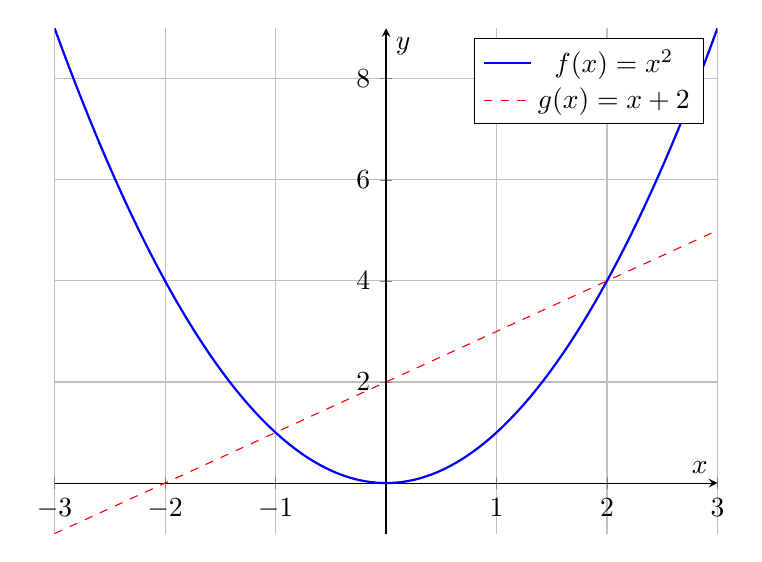
\begin{tikzpicture}
    \begin{axis}[
        axis lines = middle,
        xlabel = $x$,
        ylabel = $y$,
        grid = both,
        width=10cm,
        height=8cm,
    ]
    \addplot[domain=-3:3, samples=100, color=blue, thick] {x^2};
    \addlegendentry{$f(x)=x^2$}
    
    \addplot[domain=-3:3, samples=100, color=red, dashed] {x+2};
    \addlegendentry{$g(x)=x+2$}
    \end{axis}
\end{tikzpicture}

\end{document}
